%
% File ACL2016.tex
%

\documentclass[11pt]{article}
\usepackage{acl2016}
\usepackage{times}
\usepackage{latexsym}
\usepackage{algorithmic}
\usepackage{graphicx}

%\aclfinalcopy % Uncomment this line for the final submission
%\def\aclpaperid{***} %  Enter the acl Paper ID here

% To expand the titlebox for more authors, uncomment
% below and set accordingly.
% \addtolength\titlebox{.5in}    

\newcommand\BibTeX{B{\sc ib}\TeX}


\title{Fast, Scalable Phrase-Based SMT Decoding}

% Author information can be set in various styles:
% For several authors from the same institution:
% \author{Author 1 \and ... \and Author n \\
%         Address line \\ ... \\ Address line}
% if the names do not fit well on one line use
%         Author 1 \\ {\bf Author 2} \\ ... \\ {\bf Author n} \\
% For authors from different institutions:
% \author{Author 1 \\ Address line \\  ... \\ Address line
%         \And  ... \And
%         Author n \\ Address line \\ ... \\ Address line}
% To start a seperate ``row'' of authors use \AND, as in
% \author{Author 1 \\ Address line \\  ... \\ Address line
%         \AND
%         Author 2 \\ Address line \\ ... \\ Address line \And
%         Author 3 \\ Address line \\ ... \\ Address line}
% If the title and author information does not fit in the area allocated,
% place \setlength\titlebox{<new height>} right after
% at the top, where <new height> can be something larger than 2.25in
\author{Hieu Hoang\\
	    Moses Machine Translation CIC\\
	    {\tt hieu@moses-mt.org}
	  \And
	Nicolay Bogoychev\\
  	University of Edinburgh\\
  	10 Crichton Street\\
  	Edinburgh, Scotland, EH10 9AB\\
  {\tt s1031254@sms.ed.ac.uk}
	  \And
	Lane Schwartz\\
  	University of Illinois\\
  {\tt lanes@illinois.edu}
	  \AND
	Kenneth Heafield\\
  	University of Edinburgh\\
  {\tt kheafiel@inf.ed.ac.uk}
	  \And
	Marcin Junczys-Dowmunt\\
	Faculty of Mathematics and Computer Science \\
	Adam Mickiewicz University\\
  {\tt junczys@amu.edu.pl}
	}
	
  
\date{}

\begin{document}

\maketitle

\begin{abstract}
The utilization of statistical machine translation (SMT) has grown enormously over the last decade, many using open-source software developed by the NLP community. As commercial utilization has increased, there has been a pressing need that is optimized for their requirements. Specifically, faster phrase-based decoding, and more efficient utilization of modern multicore servers.

In this paper we re-assess the major components of phrase-based decoding and decoder implementation with particular emphasis on speed and scalability on multicore machines. The result is a drop-in replacement for the Moses decoder which is up to fifteen times faster and scales almost linearly with the number of cores. 

\end{abstract}

\section{Introduction}

SMT has been one of the outstanding success story from the NLP community in the last decade, progressing from a mostly research discipline to public useability via services such as Google Translate, Microsoft Translator Hub, as well as services and products built around offline products such as Language Weaver and the open-source Moses toolkit. The latter has spawned a cottage industry  encompassing a range of organizations and services from small language service providers seeking to reduce translation cost, to large inter-govermental organizations such as the EU and the UN that require high volume, high quality translation.

For high volume users, decoding is a largest and most critical part of the translation process which needs to be fast and efficient. However, it has been noticed that the Moses decoder, amongst others, is unable to efficiently use multiple CPU cores that are now common on modern servers~\cite{mfernandez2016boosting}. That is, the time taken to decode a test set does not substantial decrease when more cores are used, in fact, decoding time may increase when more cores are added. The problem will continue to grow as the commercial use of SMT increases and the number of CPU cores increases.

There have be speculation on the causes of the inefficiency as well as potential remedies. This paper is the first we know of that seeks to tackle this problem head on. We present an phrase-based decoder that is not only significantly faster than the Moses baseline for single-threaded operation, but is able to run multiple threads on multicore machines with only a slightly loss in linear speed. Model scores and functionality are compatible with Moses to aid comparison and ease of transition for users. All source code will be made available under an open-source license.

\subsection{Prior Work}

There are a number of open-source SMT projects, most includes a decoder. The most well known is Moses, which supports phrase-based models, hierarchical phrase-based as well as various syntax-based models. Joshua also supports hiearchical and syntax models and has recently supported phrase-based models. Phrasal supports a number of variants of the phrase-based model. CDEC supports hierarchical and syntactic models.

A number of the decoders support multithreading whilst others use alternative methods such as Hadoop or external scripts to parallelize decoding. We shall investigate the efficiency of using parallelizing decoding using the multi-processor approach. None of the decoder focus on multi-threads decoding. 

~\newcite{mfernandez2016boosting} describes running multiple processes of the Moses decoder to increase speed, treating it as a black box within a parallelization framework.

Other prior work look to optimizing specific components of decoding. ~\newcite{Chiang:2007:cl} describes the cube-pruning and cube-growing algorithm for decoding which allows the tradeoff between speed and translation quality to the adjusted with a simgle parameter. ~\newcite{Heafield-kenlm} and ~\newcite{tanaka2013efficient} describes fast, efficient datastructures for language models. ~\newcite{zens2007efficient} describes an implementation of a phrase-table for an SMT decoder that is loaded on demand, reducing the initial loading time and memory requirements. ~\newcite{junczys_tsd_2012b} extends this by compressing the on-disk phrase table and lexicalized re-ordering model resulting in impressive speed gains over previous work.

~\newcite{Heafield-mtplz} is perhaps closest in intent to this work. This takes a holistic approach to decoding, describing a novel decoding algorithm which is fis focused on better decoding speed. It also describes a number of implementation details for faster decoding. However, the decoding algorithm is only able to incorporate one stateful feature function which precludes some of the useful decoding configurations which contains multiple stateful feature functions. It does not include a load-on-demand phrase table, therefore, cannot be used in a commercial environment where phrase-table has not be filtered with a know test set for any realistic size phrase-table. Neither did this paper analyze the scalability of their work to multicore servers.

The rest of the paper will be broken up into the following sections. Next, we will describe the phrase-based model and the major implementation components, with particular emphasis on decoding speed. We will then describe modifications to improve decoding speed and present results. We conclude in the last section and discuss future work.

\section{Phrase-Based Model}

The objective of decoding is to find the target translation with the maximum probability, given a source sentence. That is, for a source sentence $s$, the objective is to find a target translation $\hat{t}$ which has the highest conditional probability $p(t | s)$. Mathematically, this is written as:
\begin{equation}
\hat{t} = \arg \max_t p( t | s )
\label{eq:argmax-factored-trans}
\end{equation}
where the \emph{arg max} function is the search. The log-linear model generalizes Equation~\ref{eq:argmax-factored-trans} to include more component models and weighting each model according to the contribution of each model to the total probability. 
\begin{equation}
\label{eq:Log-Linear}
p(t | s) 	=  \frac{1}{Z} \exp ( \sum_m \lambda_m h_m ( t, s)^{} )
\end{equation}
where $\lambda_m$ is the weight, and $h_m$ is the feature function, or `score', for model $m$. $Z$ is the partition function which can be ignored for optimization. 

\subsection{Beam Search}

A translation of a source sentence is created by applying a series of translation rules which together translate each source word once, and only once. Each partial translation is called a \emph{hypothesis}, which is created by applying a rule to an existing hypothesis. This process is called \emph{hypothesis expansion} and starts with a hypothesis that has translated no source word and ends with a completed hypothesis that has translated all source words. The highest-scoring completed hypothesis, according to the model score, is returned as  most probable translation, $\hat{t} $. Incomplete hypotheses are referred to as partial hypotheses.

Each rule translates a contiguous sequence of source words but successive translation options do not have to be adjacent on the source side, depending on the distortion limit. However, the target output is constructed strictly left-to-right from the target string of successive translation options. Therefore, successive translation options which are not adjacent and monotonic in the source causes translation reordering.

A beam search algorithm is used to create the completed hypothesis set efficiently. Partial hypotheses are organized into stacks where each stack holds a number of comparable hypotheses. Hypotheses in the same stack have the same coverage cardinality $|C|$, where $C$ is  the coverage set, $C \subseteq \{1,2,... |s| \} $ of the number of  source words translated. Therefore, $|s| + 1$ number of stacks are created for the decoding of a sentence $s$. 

There are three main optimization to the search that we shall investigate. Firstly, the search creates and destroy a large number of hypothesis objects in memory which puts a heavy burden on the operating system. We shall optimize the search algorithm to use memory pools and object pools, replacing the operating system's general purpose memory management with our own application-aware management. 

%The speed of memory access is dependent on whether the data is in the CPU cache which is a constrained resource compared to memory size, typically 20MB in the latest processors. We shall seek to re-use recently accessed information to increase likelihood of the data being in the CPU cache. 

In multiprocessor servers, the CPU cache is attached to each processor and each core. If a sentences is being decoded on one CPU is switched to another, the CPU cache on the new CPU must be repopulated, slowing down decoding. We will therefore investigate binding threads to specific cores.

Lastly, we shall investigate different stack configurations other than coverage cardinality to see whether they can improve speed and translation quality.

\subsection{Feature Functions}

Features functions are the $h_m$ in Equation~\ref{eq:Log-Linear}, calculating a score for each hypothesis.

The standard feature functions in the phrase-based model include:
\begin{enumerate}
  \item \vspace{-2 mm} log transforms translation model probabilities, $p_{TM}(t|s) $ and $p_{TM}(s|t)$, and word-based translation probabilities $p_w(t|s)$ and $p_w(s|t)$,
  \item \vspace{-2 mm} log transforms of the lexicalized re-ordering probabilities,
  \item \vspace{-2 mm} log transforms of the target language model probability $p(t)$, 
  \item \vspace{-2 mm} a distortion penalty
  \item \vspace{-2 mm} a phrase-penalty,
  \item \vspace{-2 mm} a word penalty,
  \item \vspace{-2 mm} an unknown word penalty.
\end{enumerate}
%which we have suffixed with $_{TM} $ to avoid confusion with the overall model probability $ p(t|s) $ and $ p(s|t)$. 

The first three feature functions frequently trained on data and require the feature to read the model from files. The other feature functions are simple and do not leave much room for optimization. The language model consumes a large part of decoding time, and it is for this reason that it has already been heavily optmized. We shall therefore investigate the first two feature functions for optimization.

%\subsection{Language Model}
% TODO
%
\subsection{Translation Model}

For any realistic sized phrase-based model to be used in an online situation, memory and loading time constraints requires us to use load-on-demand phrase-table implementations. Moses contains a number of such implementations with different performance characterics, we show the time take to decode 800,000 sentences for the fastest two in Figure~\ref{fig:moses-phrase-tables-time}.
\begin{figure}[h]
\centering
\begin{tabular}{cc}
{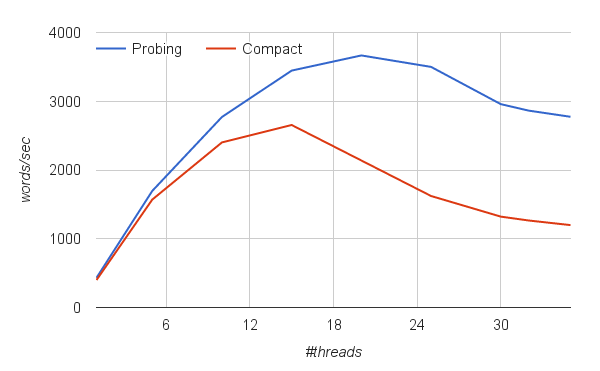
\includegraphics[scale=0.4]{moses-phrase-table.png}} 
\end{tabular}
\caption{Moses decoding time with two different phrase-table implementations}
\label{fig:moses-phrase-tables-time}
\end{figure} 
From this, it appears that the Probing phrase-table~\cite{Bogochev:Thesis:2013} has the fastest translation rule lookup, especially with large number of cores, therefore, we will concentrate exclusively on this implementation in our work as this . We will look at two main areas for phrase-table optimization specifically in relation to the Probing implementation.

We will focus on two main optimizations that differs from the current Probing phrase-table implementation and that have application to other implementations. Firstly, we will look at the \textbf{caching} of often used translation rules. The default caching framework save the most recently looked up rules. However, this caching mechanism is actually slower than re-querying the phrase-table, Table~\ref{tab:phrase-table-cache}. 
\begin{table}[h]
\small
\begin{center}
\begin{tabular}{|l|c|c|} \hline
		& No cache	& Caching \\ \hline
Decoding time  	& 2032 		& 2302 (+13\%) \\ \hline
\end{tabular}
\end{center}
\caption{Decoding time (in sec with 32 threads) when using phrase-table cache}
\label{tab:phrase-table-cache}
\end{table}
We shall explore a simpler caching mechanism that creates the cache at the start of decoding and remain static thereafter.

Secondly, the Probing phrase-table use a simple \textbf{compression} algorithm to compress the target side of the translation rule. Compression was championed as the main reason behind the speed of the Compact phrase-table but as we saw in Figure~\ref{fig:moses-phrase-tables-time}, this comes at the cost of scalability to large number of threads. We shall therefore take the opposite approach to~\newcite{junczys_tsd_2012b} and explore optimizing decoding speed by disabling compression.

\subsection{Lexicalized Reordering Model}

The lexicalized reordering model is trained on parallel data, usually requiring random lookups of the model file during decoding. Using the model can increase translation quality at the cost of longer decoding time. Efforts such as~\newcite{junczys_tsd_2012b} have been made to increase the speed of the model, with some success at low core counts, Figure~\ref{fig:moses-lex-ro}.
\begin{figure}[h]
\centering
\begin{tabular}{cc}
{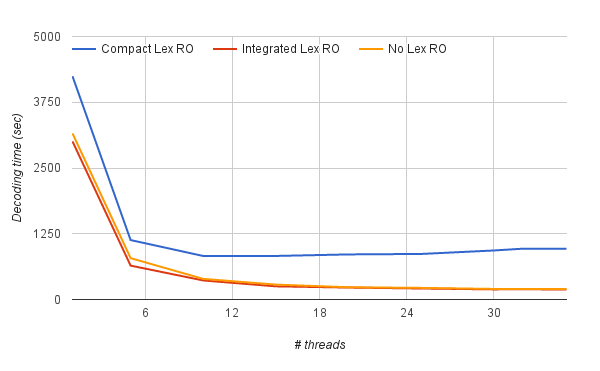
\includegraphics[scale=0.4]{moses-lex-ro.png}} 
\end{tabular}
\caption{Comparing Moses decoding time with different Lexicalized Reordering implementations}
\label{fig:moses-lex-ro}
\end{figure} 

However, the querying key to the lookup are the source and target phrase of each translation rule. Rather than storing the model separately, we shall investigate integrating the lexicalized reordering model into the translation model.


\section{Experimental Setup}

We trained a phrase-based system using the Moses toolkit with standard settings. The training data consisted of most of the publicly available Arabic-English data from Opus~\cite{tiedemann2012parallel} containing over 69 million parallel sentences, and tuned on a held out set. The phrase-table was then pruned, keeping only the top 100 entries per source phrase, according to $p(t|s)$. All models files were then binarized; the language models were binaized using KenLM~\cite{Heafield-kenlm}, the phrase table using the Probing phrase-table, lexicalized reordering model using the compact datastructure. These binary formats were choosen for their best-in-class multithreaded performance. Table~\ref{tab:model-files} gives details of the resultant sizes of the model files. For verification with a different dataset, we also occasionally used a second system trained on the French-English Europarl corpus (2m parallel sentences). 
\begin{table}[h]
\begin{center}
\begin{tabular}{|l|c|c|} \hline
		& ar-en	& fr-en \\ \hline
Phrase table  	& 17 	& 5.8 \\
Language model 	& 3.1  	& 1.8 \\ 
Lex re. model	& 2.3	& 637MB \\ \hline
\end{tabular}
\end{center}
\caption{Model sizes in GB}
\label{tab:model-files}
\end{table}
For testing decoding speed, we used a subset of the training data, Table~\ref{tab:test-sets}. The two test scenarios have differing characterics that we are interested in analyzing, ar-en have short sentences with large models while fr-en have overly long sentences with smaller models. Where we need to compare model scores, we used held out test sets.

\begin{table}[h]
\begin{center}
\small
\begin{tabular}{|l|r|r|} \hline
		& ar-en		& fr-en \\ \hline
\multicolumn{3}{|l|}{For speed testing} \\ \hline
Set name	& \multicolumn{2}{|c|}{Subset of training data} \\
\# sentences  	& 800k 		& 200k \\
\# words 	& 5.8m 		& 5.9m \\ 
Avg words/sent	& 7.3		& 29.7 \\ \hline
\multicolumn{3}{|l|}{For model score testing} \\ \hline
Set name	& OpenSubtitles	& newstest2011 \\
\# sentences  	& 2000 		& 3003 \\
\# words 	& 14,620 	& 86,162 \\ 
Avg words/sent	& 7.3		& 28.7 \\ \hline
\end{tabular}
\end{center}
\caption{Test sets}
\label{tab:test-sets}
\end{table}

Standard Moses phrase-based configurations are used, except that we use the cube-pruning algorithm~\cite{Chiang:2007:cl} with a pop-limit of 400, rather than the basic phrase-based algorithm. The cube-pruning algorithm is often employ by users who require fast decoding as it gives them the ability to trade speed with translation quality with a simple pop-limit parameter.

As a baseline, we use the latest version of the Moses decoder taken from the github repository.

For all experiments, we used a Dell PowerEdge R620 server with 16 cores, 32 hyper-threads, split over 2 physical processors (Intel Xeon E5-2650 @ 2.00GHz). The server has 380GB RAM. The operating system was Ubuntu 14.04, the code was compiled with gcc 4.8.4 and Boost library 1.59.

\section{Results}

\subsection{Optimizing Memory}

We create a dynamic memory pool which can grow as more memory is requested. The memory is not released, instead the pool can be reset in order for the memory to be re-used. We instantiate two pools for each thread, one which is never reset and another which is reset after the decoding each sentence. Datastructures are created in either pool according to their life cycle.

For critical datastructures with high churn such as hypotheses, thread-specific LIFO queues are used to recycle objects which are no longer used. This not only reduces memory wastage but re-uses recent objects which are likely to be in the CPU cache memory.

Over 24\% of the Moses decoder running time is spent on memory management and this increases when more threads are used, Table~\ref{tab:optimizing-memory}, dampening the scalability of the decoder. By contrast, our decoder spends 11\% on memory management and does not significantly increase with more cores.
\begin{table}[h]
\begin{center}
\small
\begin{tabular}{|l|c|c|c|c|} \hline
		& \multicolumn{2}{c|} {Moses}	& \multicolumn{2}{c|} {Our Work} \\ \hline
\# threads	& 1 		& 32	& 1 		& 32  \\ \hline
Memory  	& 24\%		& 39\% 	& 11\%		& 13\% \\
LM 		& 12\%	 	& 2\% 	& 47\%		& 38\% \\ 
Phrase-table	& 9\%	 	& 5\% 	& 2\%		& 4\% \\ 
Lex RO 		& 8\%	 	& 2\% 	& 2\%		& 2\% \\ 
Search 		& 2\%	 	& 0\% 	& 14\%		& 19\% \\ 
Misc/Unknown	& 45\%	 	& 39\% 	& 24\%		& 29\% \\ \hline
\end{tabular}
\end{center}
\caption{Profile of \%age decoding time}
\label{tab:optimizing-memory}
\end{table}

Figure~\ref{fig:mempool} compares the decoding time for Moses and our decoder, using the same models, parameters and test set. Our decoder is over 3 times faster with one thread, and 4.7\% faster using all cores. Like Moses, performance actually worsens after approximately 15 cores, however, the problem is not as pronounced. This gives us a better foundation on which to build further innovations for fast, multi-core decoding.
\begin{figure}[h]
\centering
\begin{tabular}{cc}
{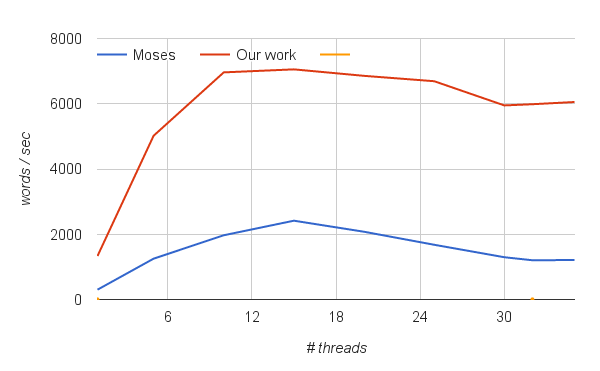
\includegraphics[scale=0.4]{mempool.png}} 
\end{tabular}
\caption{Decoding time of Moses and our decoder, using the same models}
\label{fig:mempool}
\end{figure} 

% A potential disadvantage of using memory pool is that the decoder will use more memory, however, Table~\ref{tab:memory-usage} shows that peak memory consumption are comparable.
% \begin{table}[h]
% \begin{center}
% \begin{tabular}{|l|c|c|} \hline
% 		& 1 thread	& 32 threads \\ \hline
% Moses  		& ???	 	& ??? \\
% Our work 	& ??? 		& ??? \\ \hline
% \end{tabular}
% \end{center}
% \caption{Peak Memory Usage in GB}
% \label{tab:memory-usage}
% \end{table}

\subsection{Stack Configuration}

The most popular stack configuration for phrase-based model, as implemented in Pharaoh, Moses and Joshua, has been by coverage cardinality, ie. hypotheses that have translated the same number of source words are stored in the same stack. There have been research into other stack layouts such as~\cite{ortizmartinez-garciavarea-casacuberta:2006:WMT}, and it has been noted that the decoder in~\cite{Brown:1993} uses coverage stacks, as opposed to coverage cardinality. 

We also note that distortion limit which constrains hypothesis extension is dependent on the hypothesis' coverage vector, $C$ \emph{and} the end position of most recent source word that has been translated, $e$. The distortion limit must be checked for every instance of a hypothesis and translation rule, Figure~\ref{algo:Hypothesis Expansion with Unsorted Stack}.
\begin{figure} [h]
\begin{algorithmic}
%\REQUIRE source sentence $s$, translation options
\FORALL{ $hypo$ in $stack_{|C|}$} 
  \FORALL{ translation rules}
      \IF {can-expand($C(hypo)$, $e(hypo)$, translation rule range)}
	\STATE expand hypo with translation rule $\rightarrow$ new hypo
	\STATE add new hypo to next stack
      \ENDIF
  \ENDFOR % { translation options}
\ENDFOR % { hypothesis in $stack_i$} 
\end{algorithmic}
\caption{Hypothesis Expansion with Cardinality Stacks}
\label{algo:Hypothesis Expansion with Unsorted Stack}
\end{figure}
However, by separating hypotheses into set of hypotheses (\emph{'ministacks'}) according to coverage and end position, the distortion limit only needs to be checked for each ministack, Figure~\ref{algo:Hypothesis Expansion with Sorted Stack}. Furthermore, stack pruning is done on each of these hypotheses set therefore, changing how hypotheses are grouped can affect model scores. 
\begin{figure} [h]
\begin{algorithmic}
%\REQUIRE source sentence $s$, translation options
\FORALL{ $ministack_{C, e}$ in $stack_{|C|}$} 
  \FORALL{ translation rules}
    \IF {can-expand($C$, $e$, translation rule range)}
      \FORALL{ $hypo$ in $ministack_{C, e}$} 
	\STATE expand hypo with translation rule $\rightarrow$ new hypo
	\STATE add new hypo to next ministack
      \ENDFOR
    \ENDIF
  \ENDFOR % { translation options}
\ENDFOR % { hypothesis in $stack_i$} 
\end{algorithmic}
\caption{Hypothesis Expansion with Coverage \& End Position Stacks}
\label{algo:Hypothesis Expansion with Sorted Stack}
\end{figure}
We therefore looked at the effects of three stack configurations:
\begin{enumerate}
  \item coverage cardinality,
  \item coverage,
  \item coverage and end position of most recent translated source word.
\end{enumerate}
Table~\ref{tab:stack-configuration} and Figure~\ref{fig:stack-configuration} present the tradeoff between decoding time and average model at various pop-limits.
\begin{table*}[t]
\small
\begin{center}
\begin{tabular}{|r|r|r|r|r|r|r|} \hline
Pop-limit	& \multicolumn{2}{c|}{Cardinality}	& \multicolumn{2}{c|}{Coverage}	& \multicolumn{2}{c|}{Coverage \& end pos} \\ \hline
		& Time		& Score			& Time		& Score		& Time		& Score	\\ \hline
100  		& 73		& -8.64513 		& 75		& -8.64513	& 72	& -8.64513 \\
500		& 237		& -8.59563		& 225		& -8.59563 	& 229	& -8.59612 \\
1,000	 	& 416		& -8.58700		& 397		& -8.58700	& 423	& -8.58700 \\ 
5,000 		& 1930		& -8.58165		& 1931		& -8.58165	& 2153	& -8.58098 \\ 
10,000 		& 3619		& -8.58133		& 3630		& -8.58133	& 4576	& -8.58015 \\ 
15,000 		& 4830		& -8.58130		& 5001		& -8.58130	& 7156	& -8.57999 \\ 
20,000 		& 5849		& -8.58130		& 5916		& -8.58130	& 9583	& -8.57994 \\ \hline
\end{tabular}
\end{center}
\caption{Decoding time (in secs with 32 threads) and average model scores for different stack configurations}
\label{tab:stack-configuration}
\end{table*}

\begin{figure}[h]
\centering
\begin{tabular}{cc}
{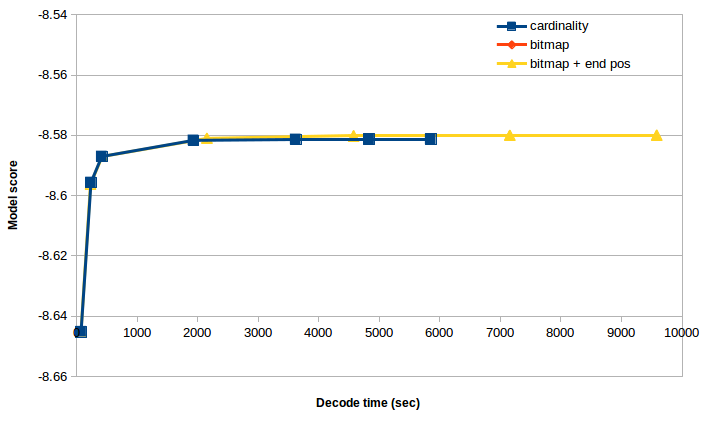
\includegraphics[scale=0.4]{stack-configuration.png}} 
\end{tabular}
\caption{Trade-off between decoding time average model scores for different stack configurations}
\label{fig:stack-configuration}
\end{figure} 
As can be seen, the model scores for all stack configurations are identical for low pop-limits parameters but grouping hypotheses into coverage \& end position produces higher model scores for higher pop-limits. It is also slower but the time/quality tradeoff is better overall with this stack configuration. For lower pop-limits this configuration is slightly slower, but not by much, therefore, we shall stick with this Configuration for the remainder of the paper.

The cube-pruning algorithm contain a further priority queue which is attached to hypotheses sets which can be independent of how hypotheses are grouped. In the Moses implementation, the priority queue is also attached to the coverage cardinality, Figure~\ref{algo:Cube Pruning with Unsorted Stack}.
\begin{figure} [h]
\begin{algorithmic}
%\REQUIRE source sentence $s$, translation options
\STATE initialize $queue_{|C|}$
\FOR{1 to pop-limit}
  \STATE get best $item$ in $queue_{|C|}$
  \STATE create hypo from $item$, coverage $C_{new}$
  \STATE add hypo to $stack_{|C_{new}|}$
  \STATE create next $items$
  \STATE add new $items$ to $queue_{|C|}$
\ENDFOR % { hypothesis in $stack_i$} 
\end{algorithmic}
\caption{Cube Pruning with Cardinality Stacks}
\label{algo:Cube Pruning with Unsorted Stack}
\end{figure}
Again, we experiment with diffirent queue configurations, having separate queues for each cardinality, coverage, and coverage \& end position. The stack configuration remained constant (coverage \& end position with pop-limit of 400).
\begin{table}[h]
\small
\begin{center}
\begin{tabular}{|r|r|r|} \hline
Queue configuration		& Time		& Score \\ \hline
Cardinality			& 192		& -8.59922 \\
Coverage			& 2,413		& -8.58635 \\
Coverage \& end position	& 7,472		& -8.58263 \\ \hline
\end{tabular}
\end{center}
\caption{Decoding time (in secs with 32 threads) and average model scores for different queue configurations}
\label{tab:queue-configuration}
\end{table}
From the results in Table~\ref{tab:queue-configuration}, using finer grain queues does results in better model scores but it is significantly slower to decode.


\subsection{Translation Model}

The Moses translation model caches the most recently queried translation rules for later re-use. This has been shown to perform badly for fast phrase-tables such as the Probing phrase-table. We explore a simple caching mechanism that populates the cache during loading with rules that translates the most common source phrases. 
\begin{table}[h]
\small
\begin{center}
\begin{tabular}{|r|r|r|} \hline
Cache size	& Decoding Time & Cache Hit \%age	\\ \hline
Before caching	& 229	& N/A	 \\
0		& 239 (+4.4\%)	& 0\% \\
1,000		& 213 (-7.0\%)	& 11\% \\
2,000		& 204 (-10.9\%)	& 13\% \\
4,000		& 205 (-10.5\%)	& 14\% \\
10,000		& 207 (-9.7\%)	& 17\% \\ \hline
\end{tabular}
\end{center}
\caption{Decoding time (in secs with 32 threads) for varying cache sizes}
\label{tab:cache}
\end{table}
The static cache does not require the overhead of managing the most recently queried lookups but there is still some overhead in using a cache. Overall however, there was over a 10\% decrease in decoding time using the optimum cache size, Table~\ref{tab:cache}.

In the second optimatization, we disable the compression. This increase the size of the binary files from 17GB to 23GB but the time saved not needing to decompress the data resulted in a 1.5\% decrease in decoding time with 1 thread and nearly 7\% when the CPU is saturated, Table~\ref{tab:compression}.
\begin{table}[h]
\small
\begin{center}
\begin{tabular}{|r|r|r|} \hline
\# threads	& Compressed pt & Non-compressed pt \\ \hline
1		& 3052	& 3006 (-1.5\%) \\
5		& 756	& 644 (-14.8\%) \\
10		& 372	& 362 (-2.7\%) \\
15		& 284	& 250 (-12.0\%) \\
20		& 244	& 227 (-7.0\%) \\
25		& 218	& 209 (-4.1\%) \\
30		& 206	& 192 (-6.8\%) \\
35		& 203	& 189 (-6.9\%) \\ \hline
\end{tabular}
\end{center}
\caption{Decoding time (in secs with 32 threads) for compressed and non-compressed phrase-tables}
\label{tab:compression}
\end{table}

\subsection{Lexicalized Reordering Model}

The lexicalized reordering model assign a probability to a translation rule, given the relative ordering of the rule in the hypothesis. 

We take a different approach by integrating the lexicalized model file into the translation model, reducing the need to query another model file. This resulted in a significant decrease in decoding time, especially with high number of cores, Figure~\ref{fig:lex-ro}. 
\begin{figure}[h]
\centering
\begin{tabular}{cc}
{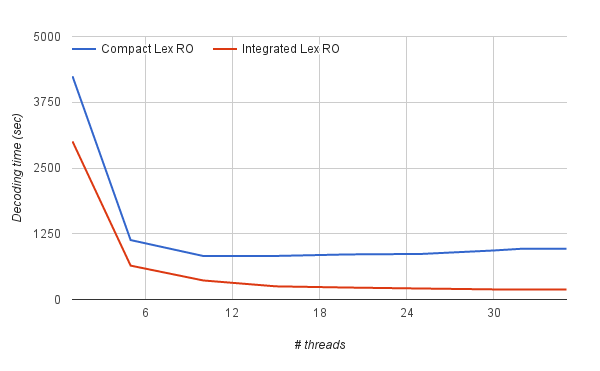
\includegraphics[scale=0.4]{lex-ro.png}} 
\end{tabular}
\caption{Decoding time with Compact Lexicalized Reordering, and integrated into a model the phrase-table}
\label{fig:lex-ro}
\end{figure} 
Integrating the lexicalized reordering model into the translation model decreases decoding time by 29\% with a single core but it is over 5 times faster using all cores. In fact, the decoding time with the integrated model is similar to that \emph{without} a lexilized reordering model. Critically for systems with large number of cores, it enables the decoder to continue to scale, making efficient use of all available cores. This is in contrast to using a separate lexicalized reordering model where decoding time flatten out and actually worsens after approximately 10 threads.

\subsection{Scalability}

\begin{figure}[h]
\centering
\begin{tabular}{cc}
{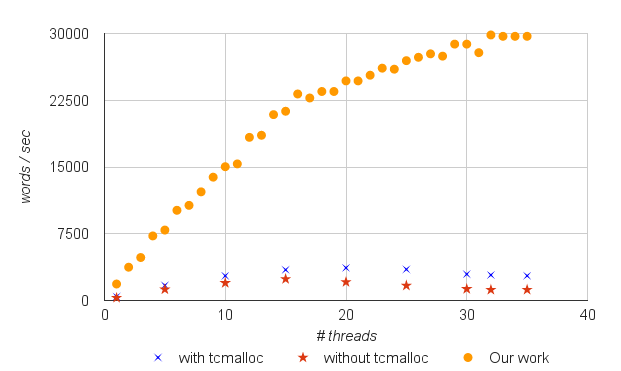
\includegraphics[scale=0.4]{scalability.png}} 
\end{tabular}
\caption{Our decoder's decoding speed}
\label{fig:speed}
\end{figure} 

Figure~\ref{fig:speed} shows decoding speed against the number of threads, measured in words translated per second. Speed increases linearly with 2 threads as each thread is run on separate physical processors. The translation rate only decrease slightly with every additional threads until 16 threads are used which produces a 12.5 times faster than single-threaded decoding. The need to share resources such as CPU cache and internal bus bandwidth is probably responsible for the non-linear increase in speed.

Since the test server only has 16 real cores, additional threads must be run on the same physical cores as existing threads. This further constrains the resources that each thread has, therefore we see a markedly lower speed increase with each additional thread once there are more than 16 concurrent threads.

Overall though, the scalability is remarkably good, the decoder is able to make full use of all real and virtual cores. When all 16 cores are saturated with 2 hyper-thread each, the decoder is 16 times faster than single-threaded decoding. It is also 4.5 times faster than Moses with a single-thread and 9.6 faster when all cores are used.

This contrast with Moses where speed increases to approximately 16 threads but then actually become slower if more threads are used, Figure~\ref{fig:moses-speed}.
\begin{figure}[h]
\centering
\begin{tabular}{cc}
{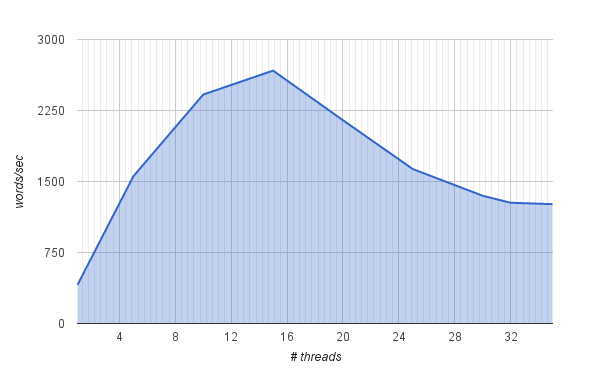
\includegraphics[scale=0.4]{moses-scalability.png}} 
\end{tabular}
\caption{Moses' decoding speed}
\label{fig:moses-speed}
\end{figure} 


\section{Other Models and Even More Cores}

??? more cores

We verify the results on a smaller French-English phrase-based model and test set containng longer sentences. The speed gain is even greater than our main testing scenario, Figure~\ref{fig:fr-en-speed}. Our decoder is 5.4 times faster than Moses with a single-thread and 14.5 faster when all cores are saturated.
\begin{figure}[h]
\centering
\begin{tabular}{cc}
{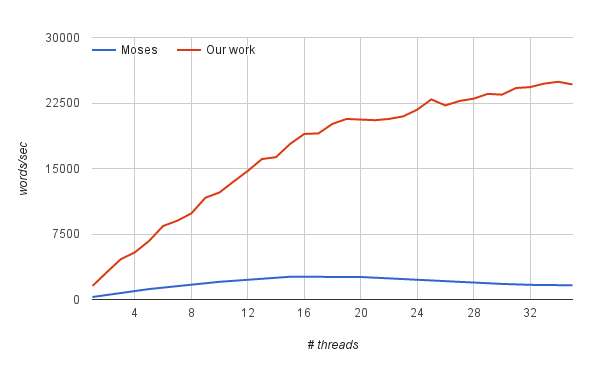
\includegraphics[scale=0.4]{fr-en-speed.png}} 
\end{tabular}
\caption{Decoding speed for fr-en model}
\label{fig:fr-en-speed}
\end{figure} 

\section{Conclusion}

We have presented a new decoder that is compatible with Moses. By studying the shortcomings of the current implementations, we are able to optimize for speed, especially for multicore operation. This has resulted in double digit gains compared to Moses on the same hardware. Our implementation is also unaffected by scalability issues that has afflicted Moses after 10-15 threads and continue to scale well for all possible cores we have tested it on.

In future, we shall investigate other major components of the decoding algorithm, particulaly the language model which has not been touched in this paper. We shall also explore the underlying reasons for the scalability issues in Moses to get a better understanding where potential performance issues can arise. This has application to other algorithms beside MT decoding. 

% \section*{Acknowledgments}
% 
% Do not number the acknowledgment section.
% This section should not be presented for the submission version.

\bibliography{acl2016,mt,more}
\bibliographystyle{acl2016}


\end{document}
